\documentclass{article}
\usepackage[final]{nips_2017}
\usepackage[utf8]{inputenc} % allow utf-8 input
\usepackage[T1]{fontenc}    % use 8-bit T1 fonts
\usepackage{hyperref}       % hyperlinks
\usepackage{url}            % simple URL typesetting
\usepackage{booktabs}       % professional-quality tables
\usepackage{amsfonts}       % blackboard math symbols
\usepackage{nicefrac}       % compact symbols for 1/2, etc.
\usepackage{microtype}      % microtypography
\usepackage{graphicx}
\title{Family kinship Recognition Using Deep Learning}

\author{
  Bruce Jianye Liu\\
  Department of Computer Science\\
  Stanford University\\
  \texttt{bruceliu@stanford.edu} \\
}

\begin{document}
% \nipsfinalcopy is no longer used

\begin{center}

\includegraphics[width=3cm, height=0.7cm]{CS230}
\end{center}

\maketitle

\section{Problem Description}
Half of genetic informaiton is passed down from parents to children. If looking
at family photos, human eyes could easily tell the simliarity faces. As
computer vision performance developed, we could use deep learning to recognise
the kinship. Possible applications could be missing-children and parents
matching, personal photos sharing among families, socal networking apps,
searching lost sibling/relatives, crime investigation.

\section{Challenges}
It might be hard to achieve higher accuracy since people without any family kinship would look simliar to each other.

\section{Dataset}
We are going to use Families In The Wild (FIW) Database. FIW is the largest and
most comprehensive database available for kinship recognition. It is made up of
11,932 natural family photos of 1,000 families. It includes 656,954 image pairs
divided into parent-child pair-wise types -- father-daughter (F-D), father-son
(F-S), mother-daughter (M-D), mother-son (M-S) and siblings pairs types --
brother-brother (B-B), sister-sister (S-S).

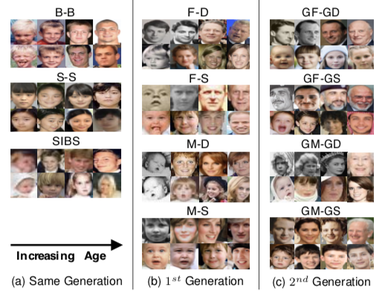
\includegraphics{facepairs}

There are another smaller family dataset KinFaceW-I and KinFaceW-II, which
includes 533 pairs of parent-child type images.

We divided 95 of the images as training set, 5 percent as test set.

\section{Models and Evaluation}
we use classifier to indicate the kinship distance between two faces. The output layer could be softmax function of {p-c, sibling, no-relationship}.



\section*{References}
\medskip
\small
[1] Robinson, J.P., Shao, M., Wu, Y.\ \& Fu, Y.\ (2017) Families in the Wild (FIW): Large-Scale Kinship Image Database and Benchmarks \ arXiv:1604.02182 [cs.CV]

\end{document}
